%
% LaTeX Report Assignment 4
% Applied Programming Lab EE2703
% Ayush Jamdar EE20B018 
%


\documentclass[11pt, a4paper]{article}
\usepackage{graphicx}
\usepackage{amsmath}
\usepackage{listings}
\usepackage[]{courier}
%\usepackage{hyperref}


\title{Assignment 10: Convolution}

\author{Ayush Jamdar EE20B018} % Author name


\begin{document}		
		
\maketitle % Insert the title, author and date
\section{Aim}
The goal is to implement linear and circular convolution using methods of scientific computing. 
Convolution is defined as 
$$y[n]=\sum_{k=-\infty}^{\infty}x[n-k]h[k]$$
In Fourier domain, 
$$Y[m]=X[m]H[m]$$

\section{The Assignment}
\subsection{The FIR Filter}
The \texttt{h.csv} file is given on Moodle. It contains the FIR $h[n]$. Then I take a DFT using the \texttt{sig.freqz()} function. The magnitude and phases are plotted (Figure 1 and 2). The code follows. 
\begin{verbatim}
with open("h.csv") as f:
    h = np.loadtxt(f, delimiter=",")

# plotting the filter response
# USE: scipy.signal.freqz()
w, H = sig.freqz(h)  # takes the fourrier transform of the filter
plt.plot(w, 20 * np.log10(abs(H)))
plt.xlabel("Frequency (rad/sample)")
plt.ylabel("Magnitude (dB)")
plt.title("Magnitude Response")
plt.grid()
plt.savefig("h.png")
plt.show()
\end{verbatim}

\begin{figure}[!tbh]
   	\centering
  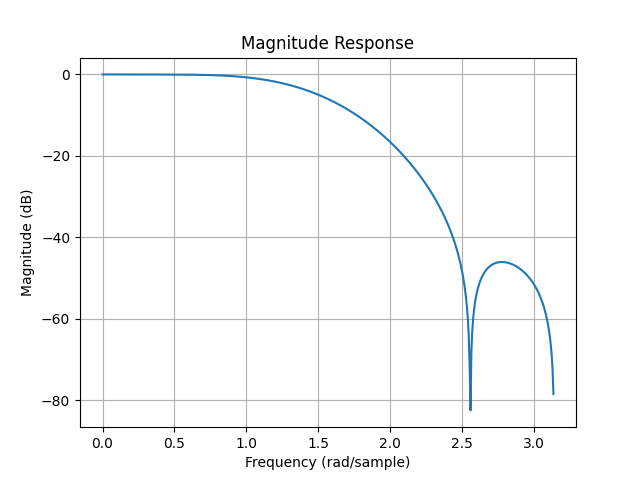
\includegraphics[scale=0.5]{h.png} 
    \caption{Magnitude Response} 	
   \end{figure}  
   
\begin{figure}[!tbh]
   	\centering
  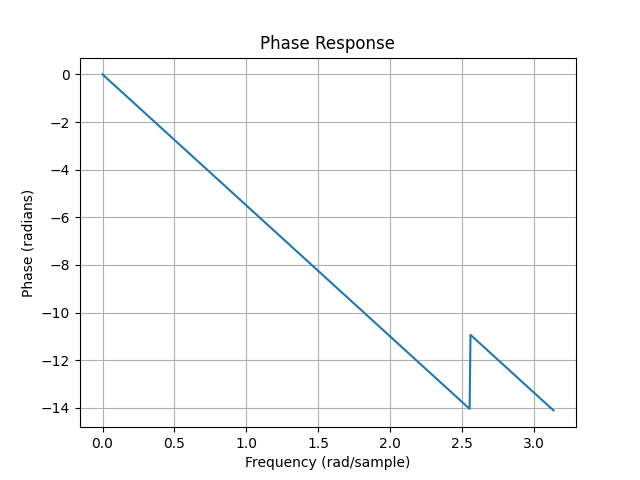
\includegraphics[scale=0.5]{h_phase.png} 
    \caption{Phase Response} 	
   \end{figure}  
   
\subsection{Input Signal}
$$x[n] = cos(0.2\pi n)+cos(0.85\pi n)$$
$n$ varies from $1$ to $2^{10}$. The sequence is generated and plotted. 

\begin{figure}[!tbh]
   	\centering
  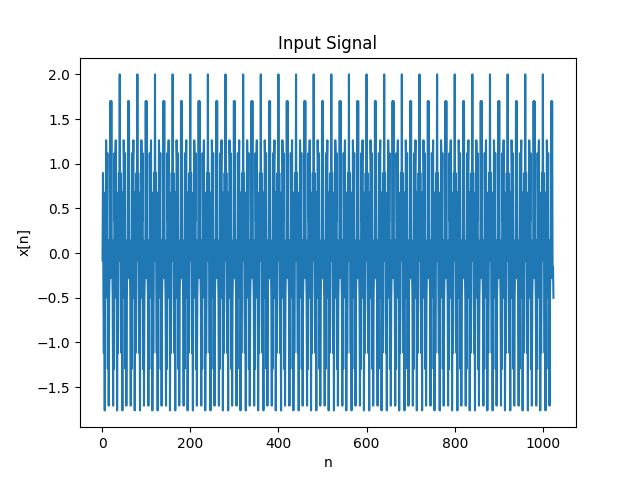
\includegraphics[scale=0.5]{x.png} 
    \caption{Input Signal} 	
   \end{figure}  
   
\subsection{Linear Convolution}
The output of the LTI system is the convolution of input and impulse response. A computationally intensive idea is nested for loops.  
\begin{verbatim}
y = np.zeros(len(x))
for i in range(len(x)):
    for j in range(len(h)):
        if i + j < len(x):
            y[i] += x[i + j] * h[j]

plt.plot(n, y)
plt.xlabel("n")
plt.ylabel("y[n]")
plt.title("Output Signal")
plt.savefig("y.png")
plt.grid()
plt.show()
\end{verbatim}

The high frequency (0.85) is filtered out. 

\subsection{Circular Convolution}
I zero pad the FIR such that \texttt{x} and \texttt{h} are now equally long. Then their DFTs are multiplied, IDFT gives the required output. It looks the same as the one 
\begin{verbatim}
Y = np.fft.fft(x) * np.fft.fft(np.concatenate((h, np.zeros
   (len(x) - len(h)))))
y_circ = np.fft.ifft(Y)
plt.plot(n, y_circ)
plt.xlabel("n")
plt.ylabel("y[n]")
plt.title("Output Signal - Circular Convolution")
plt.savefig("y_circ.png")
plt.grid()
plt.show()
\end{verbatim}

\begin{figure}[!tbh]
   	\centering
  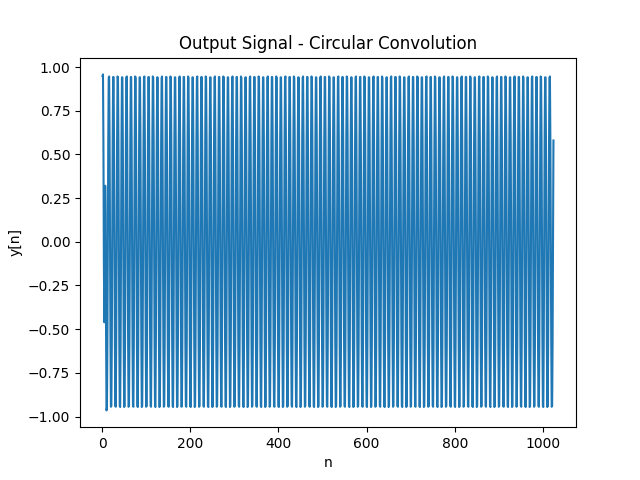
\includegraphics[scale=0.5]{y_circ.png} 
    \caption{Output Signal} 	
   \end{figure}  

\subsection{Linear Convolution Using Circular Convolution}
This is tricky. Our FIR was 12 samples long (P = 12). To extend it to $2^m$, we need to add 4 more zeros. Hence it is now 16 samples. This is \texttt{h\_with\_zeros}. Now, the input signal had 1024 samples. I make sections of \texttt{x} such that each is $L = 64$ long. In our case, x had $2^m$ samples already, which may not be the case always. Hence, the line to zero pad. Now begins the circular convolution algorithm. The logic is explained in the assignment how $y$ will have $N$ wrong values and how it obtains the correct numbers from the next computation. I take real values of the output for the plot's sake and plot the first 1024 values of \texttt{y\_circ\_conv} (as n is defined that way). Note that the length of \texttt{y\_circ\_conv} is 1039, which is \texttt{len(x) + len(h) - 1}.   

each succeeding convolution adds to the previous values of \texttt{y}.

\begin{verbatim}
P = len(h)
n1 = int(np.floor(np.log2(P))) + 1  # process to pad zeros to h
h_with_zeros = np.concatenate((h, np.zeros(int((2**n1)) - P)))
len_h = len(h_with_zeros)  # = P
L = int(np.floor(len(x) / 2**n1))  # length of each section of x
x_with_zeros = np.concatenate((x, np.zeros(L * (int(2**n1)) -
   len(x))))
y_circ_conv = np.zeros(
    len(x_with_zeros) + len(h_with_zeros) - 1
)  # using property of convolution, we know the length

for i in range(L):
    x_ = np.concatenate(
        (x_with_zeros[i * len_h : (i + 1) * len_h],
         np.zeros(len_h - 1))
    )
    y_circ_conv[i * len_h : (i + 1) * len_h + len_h - 1] +=
     np.fft.ifft(
        np.fft.fft(x_)
        * np.fft.fft(
            np.concatenate((h_with_zeros, np.zeros(len(x_)
             - len(h_with_zeros))))
        )
    ).real

"""
if .real is not used, the following error is thrown:
    numpy.core._exceptions.UFuncTypeError: Cannot cast
     ufunc 'add' output from dtype('complex128') to 
     dtype('float64') with casting rule 'same_kind' 
"""
plt.plot(n, (y_circ_conv[:1024]).real)  # as n goes from 1 to 2**10
plt.xlabel("n")
plt.ylabel("y[n]")
plt.title("Linear Convolution from Circular Convolution")
plt.savefig("lin_from_cir.png")
plt.grid()
plt.show()

\end{verbatim}

\begin{figure}[!tbh]
   	\centering
  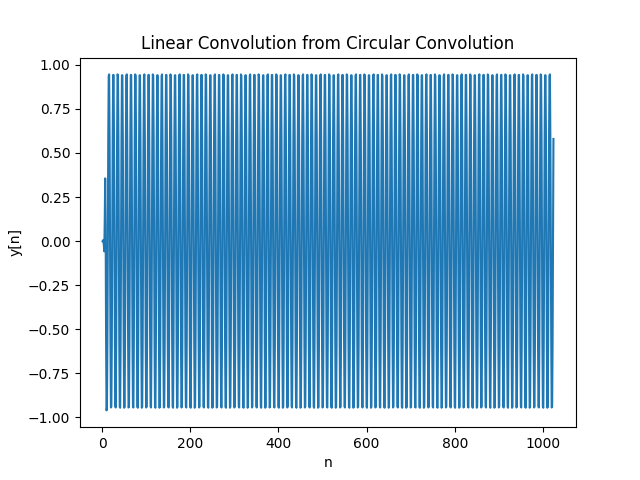
\includegraphics[scale=0.5]{lin_from_cir.png} 
    \caption{Liinear from Circular Convolution} 	
   \end{figure}  
   
\subsection{Circular Correlation}
Open the Zadoff - Chu sequence file, obtain the complex numbers from that. 
\begin{verbatim}
with open("x1.csv") as f:
    csvreader = csv.reader(f)
    lines = np.array([row for row in csvreader])

# print(lines, type(lines), lines.shape)
# this tells that the array is a numpy array 
  and numbers are given as a+ib
# we need to convert them to complex numbers
zandoff_chu_seq = []
for line in lines:
    try:
        a, bi = line[0].split("+")
        a = float(a)
        bi = float(bi[:-1])  # leaving the i
    except ValueError:
        try:
            if line[0][0] == "-":
                _, a, bi = line[0].split("-")
            else:
                a, bi = line[0].split("-")
            a = float(a)
            bi = -float(bi[:-1])  # leaving the i
        except ValueError:
            a = float(line[0])  # there is a 1 in the list
            bi = 0.0

    zandoff_chu_seq.append([a + 1j * bi])

\end{verbatim}


Now, compute correlation. 
\begin{verbatim}
zandoff_chu_seq = np.array(zandoff_chu_seq)
# print(zandoff_chu_seq, len(zandoff_chu_seq), zandoff_chu_seq.shape)
# correlation of this sequence with a shifted version of itself
shifted_zandoff_chu_seq = np.roll(zandoff_chu_seq, 5)
correlation = np.fft.ifftshift(
    np.correlate(shifted_zandoff_chu_seq[:, 0], 
    zandoff_chu_seq[:, 0], "full")
)
print(len(correlation))
plt.plot(np.arange(0, len(correlation)), abs(correlation), "ro")
plt.xlabel("n")
plt.ylabel("correlation")
plt.xlim(0, 30)
plt.title("Correlation of Zadoff-Chu Sequence")
plt.savefig("correlation.png")
plt.grid()
plt.show()
\end{verbatim}

As expected, it gives a peak at 5.
\begin{figure}[!tbh]
   	\centering
  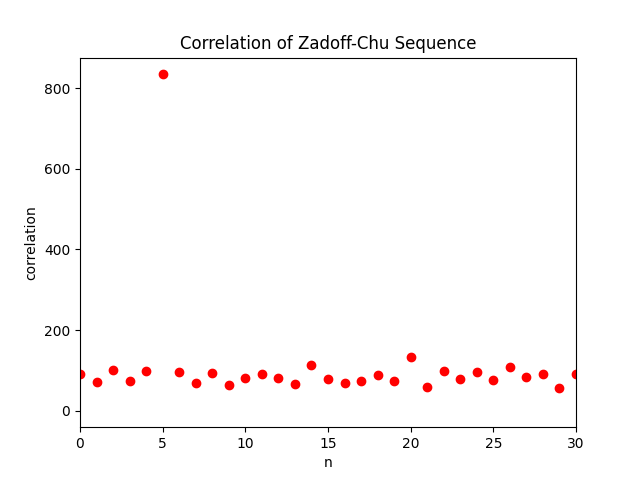
\includegraphics[scale=0.5]{correlation.png} 
    \caption{Correlation} 	
   \end{figure}  
   
   
\section{Conclusion}
Direct computation of linear convolution has a high time complexity. A faster way to do this is using DFTs. Also, circular convolution can be used to compute the output at a much lower ($log(n)$) complexity. Towards the end, an interesting property of the Zadoff Chu sequence was studied that it shows a peak in its auto-correlation at the point corresponding to the shift.

\end{document}